\documentclass{article}
\usepackage{amsfonts,enumerate}
\usepackage{graphicx}
\usepackage{listings}
\usepackage{xcolor}

%%%%%%%%%%%%%%%%%%%%%%%%%%%%%%%%%%%%%%%%%%%%%%%%%%%%%%%%%%%%%%%%
%  6.826 (POCS Seminar) macro file for handouts and problem sets.
%
% You should save this file as handout.tex
%
% Your main LaTeX file should look like this:
%
%        \documentstyle[12pt]{article}
%
%        %%%%%%%%%%%%%%%%%%%%%%%%%%%%%%%%%%%%%%%%%%%%%%%%%%%%%%%%%%%%%%%%
%  6.826 (POCS Seminar) macro file for handouts and problem sets.
%
% You should save this file as handout.tex
%
% Your main LaTeX file should look like this:
%
%        \documentstyle[12pt]{article}
%
%        %%%%%%%%%%%%%%%%%%%%%%%%%%%%%%%%%%%%%%%%%%%%%%%%%%%%%%%%%%%%%%%%
%  6.826 (POCS Seminar) macro file for handouts and problem sets.
%
% You should save this file as handout.tex
%
% Your main LaTeX file should look like this:
%
%        \documentstyle[12pt]{article}
%
%        \input{handout}
%%%%%%%%%%%%%%%%%%%%%%%%%%%%%%%%%%%%%%%%%%%%%%%%%%%%%%%%%%%%%%%%

\oddsidemargin 0in
\evensidemargin 0in
\marginparwidth 40pt
\marginparsep 10pt
\topmargin 0pt
\headsep 0in
\headheight 0in
\textheight 8.5in
\textwidth 6in
\brokenpenalty=10000

% \handout{number}{date}{title}

\newcommand{\handout}[3]{


\begin{center}
\rule{\textwidth}{.0075in} \\
\rule[3mm]{\textwidth}{.0075in}\\

CMU 17-651\hfill Models of Software Systems\hfill Fall 2018\\[3ex]

{\Large\bf #3}\\[3ex]

Dario A Lencina-Talarico \hfill {\bf Handout #1} \hfill #2

\rule{\textwidth}{.0075in} \\
\rule[3mm]{\textwidth}{.0075in} \\
\end{center}

}

% \homework{number}{date}{title}{due-date}
\newcommand{\homework}[4]{

\begin{center}
\rule{\textwidth}{.0075in} \\
\rule[3mm]{\textwidth}{.0075in}\\

CMU 17-651\hfill Models of Software Systems\hfill Fall 2018\\[3ex]

{\Large\bf #3} \\[3ex]

Dario A Lencina Talarico \hfill  #1  \hfill Due: #2\\

\rule{\textwidth}{.0075in} \\
\rule[3mm]{\textwidth}{.0075in} \\
\end{center}

%\noindent
%{\bf Due date: #4}

}

% \solutionset{number}{date}{title}{due-date}
\newcommand{\solutionset}[4]{

\begin{center}
\rule{\textwidth}{.0075in} \\
\rule[3mm]{\textwidth}{.0075in}\\

CMU 17-651\hfill Models of Software Systems\hfill Fall 2016\\[3ex]

{\Large\bf #3} \\[3ex]

Garlan  \hfill  Solutions for Homework #1  \hfill  #2\\

\rule{\textwidth}{.0075in} \\
\rule[3mm]{\textwidth}{.0075in} \\
\end{center}

%\noindent
%{\bf Due date: #4}

}

% \problem{problem-number}
\newcommand{\problem}[1]{
\vspace{2ex}
\noindent
{\bf Problem #1.}

}

% \solution{solution-number}{points}
\newcommand{\solution}[2]{
\vspace{3ex}
\noindent
{\bf Problem #1}  (#2 points)

}

\newcommand{\cscomment}{
\vspace{1ex}
\noindent Comments: }

% \parts{part-alphabet}{points}
\newcommand{\parts}[2]{
\vspace{2ex}
\noindent
{\bf (#1)}  (#2 points)

}

% \problems{problems-number}{points}
\newcommand{\problems}[2]{
\vspace{3ex}
\noindent
{\bf Problem #1}  (#2 points)

}

\newenvironment{symbolfootnotes}{\def\thefootnote{\fnsymbol{footnote}}}{}

%%%%%%%%%%%%%%%%%%%%%%%%%%%%%%%%%%%%%%%%%%%%%%%%%%%%%%%%%%%%%%%%

\oddsidemargin 0in
\evensidemargin 0in
\marginparwidth 40pt
\marginparsep 10pt
\topmargin 0pt
\headsep 0in
\headheight 0in
\textheight 8.5in
\textwidth 6in
\brokenpenalty=10000

% \handout{number}{date}{title}

\newcommand{\handout}[3]{


\begin{center}
\rule{\textwidth}{.0075in} \\
\rule[3mm]{\textwidth}{.0075in}\\

CMU 17-651\hfill Models of Software Systems\hfill Fall 2018\\[3ex]

{\Large\bf #3}\\[3ex]

Dario A Lencina-Talarico \hfill {\bf Handout #1} \hfill #2

\rule{\textwidth}{.0075in} \\
\rule[3mm]{\textwidth}{.0075in} \\
\end{center}

}

% \homework{number}{date}{title}{due-date}
\newcommand{\homework}[4]{

\begin{center}
\rule{\textwidth}{.0075in} \\
\rule[3mm]{\textwidth}{.0075in}\\

CMU 17-651\hfill Models of Software Systems\hfill Fall 2018\\[3ex]

{\Large\bf #3} \\[3ex]

Dario A Lencina Talarico \hfill  #1  \hfill Due: #2\\

\rule{\textwidth}{.0075in} \\
\rule[3mm]{\textwidth}{.0075in} \\
\end{center}

%\noindent
%{\bf Due date: #4}

}

% \solutionset{number}{date}{title}{due-date}
\newcommand{\solutionset}[4]{

\begin{center}
\rule{\textwidth}{.0075in} \\
\rule[3mm]{\textwidth}{.0075in}\\

CMU 17-651\hfill Models of Software Systems\hfill Fall 2016\\[3ex]

{\Large\bf #3} \\[3ex]

Garlan  \hfill  Solutions for Homework #1  \hfill  #2\\

\rule{\textwidth}{.0075in} \\
\rule[3mm]{\textwidth}{.0075in} \\
\end{center}

%\noindent
%{\bf Due date: #4}

}

% \problem{problem-number}
\newcommand{\problem}[1]{
\vspace{2ex}
\noindent
{\bf Problem #1.}

}

% \solution{solution-number}{points}
\newcommand{\solution}[2]{
\vspace{3ex}
\noindent
{\bf Problem #1}  (#2 points)

}

\newcommand{\cscomment}{
\vspace{1ex}
\noindent Comments: }

% \parts{part-alphabet}{points}
\newcommand{\parts}[2]{
\vspace{2ex}
\noindent
{\bf (#1)}  (#2 points)

}

% \problems{problems-number}{points}
\newcommand{\problems}[2]{
\vspace{3ex}
\noindent
{\bf Problem #1}  (#2 points)

}

\newenvironment{symbolfootnotes}{\def\thefootnote{\fnsymbol{footnote}}}{}

%%%%%%%%%%%%%%%%%%%%%%%%%%%%%%%%%%%%%%%%%%%%%%%%%%%%%%%%%%%%%%%%

\oddsidemargin 0in
\evensidemargin 0in
\marginparwidth 40pt
\marginparsep 10pt
\topmargin 0pt
\headsep 0in
\headheight 0in
\textheight 8.5in
\textwidth 6in
\brokenpenalty=10000

% \handout{number}{date}{title}

\newcommand{\handout}[3]{


\begin{center}
\rule{\textwidth}{.0075in} \\
\rule[3mm]{\textwidth}{.0075in}\\

CMU 17-651\hfill Models of Software Systems\hfill Fall 2018\\[3ex]

{\Large\bf #3}\\[3ex]

Dario A Lencina-Talarico \hfill {\bf Handout #1} \hfill #2

\rule{\textwidth}{.0075in} \\
\rule[3mm]{\textwidth}{.0075in} \\
\end{center}

}

% \homework{number}{date}{title}{due-date}
\newcommand{\homework}[4]{

\begin{center}
\rule{\textwidth}{.0075in} \\
\rule[3mm]{\textwidth}{.0075in}\\

CMU 17-651\hfill Models of Software Systems\hfill Fall 2018\\[3ex]

{\Large\bf #3} \\[3ex]

Dario A Lencina Talarico \hfill  #1  \hfill Due: #2\\

\rule{\textwidth}{.0075in} \\
\rule[3mm]{\textwidth}{.0075in} \\
\end{center}

%\noindent
%{\bf Due date: #4}

}

% \solutionset{number}{date}{title}{due-date}
\newcommand{\solutionset}[4]{

\begin{center}
\rule{\textwidth}{.0075in} \\
\rule[3mm]{\textwidth}{.0075in}\\

CMU 17-651\hfill Models of Software Systems\hfill Fall 2016\\[3ex]

{\Large\bf #3} \\[3ex]

Garlan  \hfill  Solutions for Homework #1  \hfill  #2\\

\rule{\textwidth}{.0075in} \\
\rule[3mm]{\textwidth}{.0075in} \\
\end{center}

%\noindent
%{\bf Due date: #4}

}

% \problem{problem-number}
\newcommand{\problem}[1]{
\vspace{2ex}
\noindent
{\bf Problem #1.}

}

% \solution{solution-number}{points}
\newcommand{\solution}[2]{
\vspace{3ex}
\noindent
{\bf Problem #1}  (#2 points)

}

\newcommand{\cscomment}{
\vspace{1ex}
\noindent Comments: }

% \parts{part-alphabet}{points}
\newcommand{\parts}[2]{
\vspace{2ex}
\noindent
{\bf (#1)}  (#2 points)

}

% \problems{problems-number}{points}
\newcommand{\problems}[2]{
\vspace{3ex}
\noindent
{\bf Problem #1}  (#2 points)

}

\newenvironment{symbolfootnotes}{\def\thefootnote{\fnsymbol{footnote}}}{}
\newcommand{\Until}{\,\mathcal{U}\,}
\newcommand{\Next}{\bigcirc}
\begin{document}

\homework{}{30 November 2018}{Homework \#14: Probabilistic Model Checking}{}


%% PRISM CODE LISTING *********************************************

\definecolor{prismgreen}{rgb}{0, 0.6, 0}

\lstdefinelanguage{Prism}{ % syntax highlight via font
        basicstyle=\color{black}\scriptsize\sffamily, % small true type font (like courier)
        keywords= {bool,C,ceil,const,ctmc,double,dtmc,endinit,endmodule,endrewards,endsystem,F,false,floor,formula,G,global,I,init,int,label,max,mdp,min,module,nondeterministic,P,Pmin,Pmax,prob,probabilistic,R,rate,rewards,Rmin,Rmax,S,stochastic,system,true,U,X, player, endplayer},
        keywordstyle={\bfseries\color{black}},
        numberstyle=\tiny\color{black},
        belowcaptionskip=\baselineskip,
        comment=[l] {//}, morecomment=[s]{/*}{*/}, % single and multi-line
        commentstyle= \color{prismgreen}, % dark green
        tabsize=4, % tab treatment (going to be fixed in Prism)
        captionpos=b, % put captions at the bottom
        escapechar=@, % write LaTeX comments escaped by @ symbol
        belowcaptionskip=0em,
        belowskip=0em,
}


%\begin{tabular}{cc}
%\begin{minipage}[l]{0.6\textwidth}

%\end{minipage}

%&
%\begin{minipage}[t]{0.4\textwidth}
%\end{minipage}

%\\

%\end{tabular}

\begin{enumerate}
\item Probabilistic models augment normal state machines by associating probabilities with transitions. List one advantage of having models with this additional level of expressiveness. List one disadvantage.\\
  Removes the non-determinism from transitions and instead proposes a probabilistic approach. This allows us to reason about the probability of different conditions to occur in a more mathematical and predictible way.\\
  Each transition must have a P associated with it, sometimes it might be not obvious what the probability is.\\
\item Consider the following probabilistic model, that emulates a 6-sided die with a fair coin. Starting from state 0 ({\tt s=0}), a coin is tossed at every step, and there is a 50\% chance of taking each of the two possible choices. The process finishes when you reach one of the values of the die on the right-hand side (encoded in variable {\tt d} in the PRISM listing):

\begin{figure}[!h]
\centering
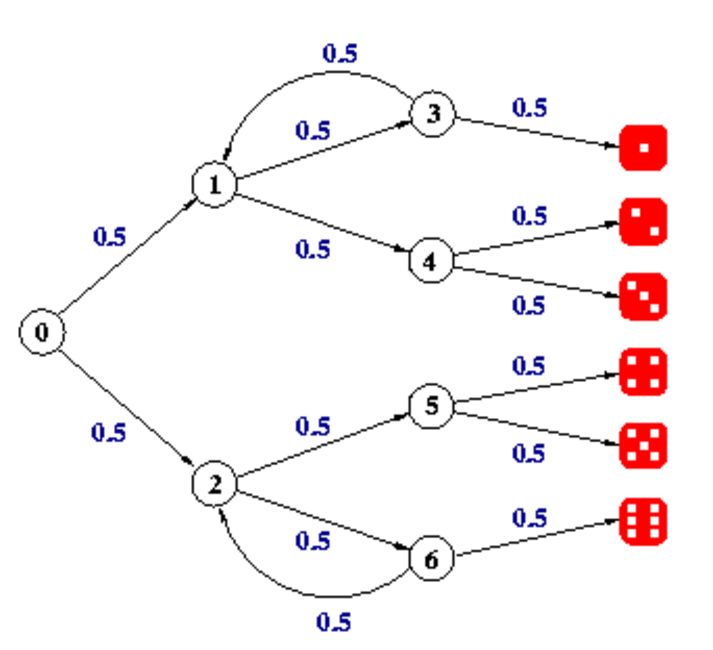
\includegraphics[width=0.5\textwidth]{dice}
\end{figure}


For each of the following questions/statements: (a) write a PCTL temporal formula to obtain the answer, (b) write the result obtained by checking the PCTL formula with the PRISM tool, and (c) briefly explain why that result was obtained.
\begin{enumerate}
\item What is the probability of rolling a 6? \\
  \begin{center}
    P=? [ F d=6 ] \\
    Result: \\
    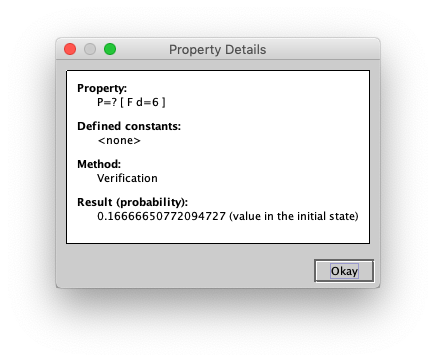
\includegraphics[width=0.5\textwidth]{p6}\\
  \end{center}
  0.16 makes sense as the probability of rolling any side of a die is $\frac{1}{6}$ 
\item Are the probability of rolling a 1 and a 4 the same? \\
  P=? [ F d=1 ] PRISM returned 0.16...\\
  P=? [ F d=4 ] PRISM returned 0.16...\\
  Yes, P is the same, and this is good because it means that the model used to simulate the model is good since by definition, rolling each side of the die should have the same exact probability unless the die is fixed :).\\
\item With probability 1, the value of the die will be 0 until state 7 is reached.
  \begin{center}
    P=? [ (d=0) U (s=7) ] \\
    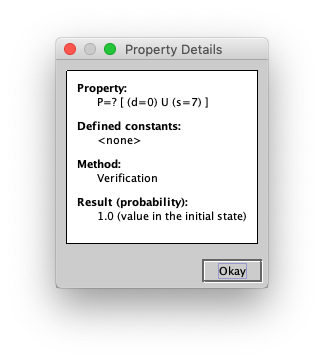
\includegraphics[width=0.5\textwidth]{s3d4}
  \end{center}
  This makes sense as d is initialized as 0 and upon reaching the tree leafs which is s=7 were d transitions to a value between 1..6 to represent the die sides.\\
\item What is the probability of eventually reaching state 3?
  \begin{center}
    $P=? [ F s=3]$\\
    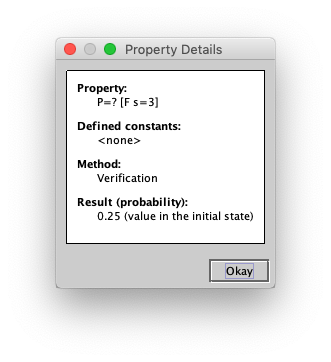
\includegraphics[width=0.5\textwidth]{p2d}\\
  \end{center}
  Makes sense since the path to 3 requires to get from 0 -> 1 witch P is 0.5 and then from 1 to 3 which P value is 0.5, if we multiply the P's = 0.5 * 0.5 = 0.25
\item What is the probability of eventually reaching state 3 and rolling a 2?
    \begin{center}
     $P=? [ (F s=3) \& (F d=2) ]$\\
    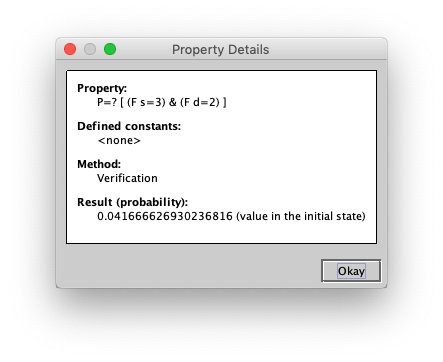
\includegraphics[width=0.5\textwidth]{s3d2}\\
    \end{center}
\item What is the probability of eventually reaching state 3 and rolling a 5?
  \begin{center}
     $P=? [ (F s=3) \& (F d=5) ]$\\
    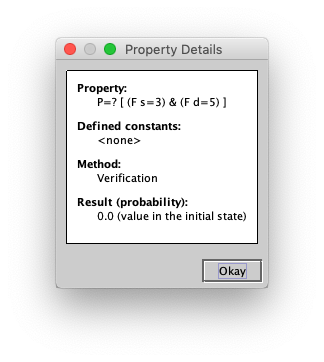
\includegraphics[width=0.5\textwidth]{s3d5}\\
  \end{center}
  Makes sense as it is not possible to reach d=5 after going through s=3.\\
\end{enumerate}

\item Consider the client-server example seen in class. For each of the following questions/statements: (a) write a PCTL temporal formula to obtain the answer, (b) write the result obtained by checking the PCTL formula with the PRISM tool, and (c) briefly explain why that result was obtained.

\begin{enumerate}
\item What is the probability that the client will acquire the channel in the first attempt, and that the server will fail to reply? \\
  \begin{center}
     $P=? [(X sc=c\_acquired) \& (F ss=s\_reply\_fail)]$\\
    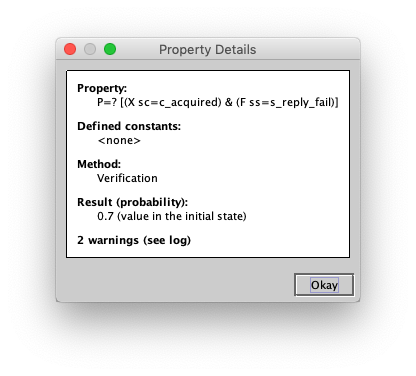
\includegraphics[width=0.5\textwidth]{hw14p31}\\
  \end{center}
  I do not think that my equation is correct as I would expect the P to be lower than 0.7 because the probability of failing to send a message is 0.5.\\
\item  The server will never attempt to reply (successfully or unsuccessfully) until a request has successfully been sent by the client.
   \begin{center}
     $P=? [(!ss=s\_reply\_success\: U\:sc=c\_send\_success) \& (!ss=s\_reply\_fail\: U\: sc=c\_send\_success)]$\\
     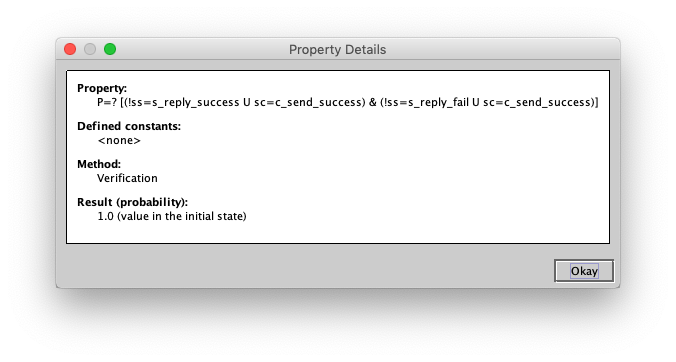
\includegraphics[width=0.5\textwidth]{hw14p32}\\
     The probability of the system respecting the premise is 1 which means that it will be always be followed, this makes sense as it is not possible for the server to reply until receiving a request, I am sure that it is possible to write down a more compact version of this equation.\\
  \end{center}
\end{enumerate}

\end{enumerate}

\end{document}
